\section{Kinematics}
\label{ch:kinematics}

In order to control the UAV with regards to where the camera is pointing, a kinematic model that maps the camera focus to the UAV position and attitude is needed. An overview of the kinematic model for the UAV will be given here, as well as the method used for calculating the camera footprint based on the UAVs attitude states.

\subsection{UAV States}
The position of the UAV will be given in reference frame \{n\} using the North East Down (NED) coordinate frame:

\begin{equation}
	\bm{p}_{b/n}^n =
	\begin{bmatrix}
		N \\ E \\ D
	\end{bmatrix}
	=
	\begin{bmatrix}
		x_n \\ y_n \\ z_n
	\end{bmatrix}
\end{equation}

The attitude of the UAV will be given as Euler-angles:

\begin{equation}
	\bm{\Theta}_{nb} = 
	\begin{bmatrix}
		\phi \\ \theta \\ \psi
	\end{bmatrix}
\end{equation}
	
where $\phi$ represents the roll angle, $\theta$ the pitch angle and $\psi$ the heading angle. The attitude angles have the corresponding angular velocities denoted $p$, $q$ and $r$ respectively. In all the simulations done in this paper there will be no wind, and it may therefore be assumed that the course angle $\chi$ is equal to the heading $\psi$.


\subsection{Camera Position}

\begin{figure}
	\import{/}{kinematic_figure.tex}
	\caption{Illustration of how the aircraft attitude influence the camera position.}
	\label{fig:camera_kinematics}
\end{figure}
	
The position of the camera center point is coupled with the attitude of the aircraft. Figure \ref{fig:camera_kinematics} shows how the position of the camera is affected by the attitude $\bm{\Theta}_{nb}$ in the body frame \{b\}, and the height $z_n$ in the NED frame \{n\}. This model assumes flat earth. The camera position in the body frame \{b\} is expressed as

\begin{equation} \label{eq:camera_pos}
	\bm{c}_b^b =
	\begin{bmatrix}
		c_{x/b}^b \\
		c_{y/b}^b
	\end{bmatrix}
	=
	\begin{bmatrix}
		z_n tan(\theta) \\
		z_n tan(\phi)
	\end{bmatrix}.
\end{equation}

In order to express the camera position $\bm{c}_b^b$ in \{n\}, the heading $\psi$ of the aircraft must be taken into consideration. This is done by rotating the point $\bm{c}_b^b$ with the rotational matrix $\bm{R}_{z,\psi}$:

\begin{equation} \label{eq:body_ned_rotate}
	\bm{c}_b^n =
	\begin{bmatrix}
		c_{x/b}^n \\
		c_{y/b}^n
	\end{bmatrix}
	= \bm{R}_{z,\psi} \bm{c}_b^b,
\end{equation}

where:

\begin{equation}
	\bm{R}_{z,\psi} = 
	\begin{bmatrix}
		cos(\psi) & -sin(\psi) & 0 \\
		sin(\psi) & cos(\psi) & 0 \\
		0 & 0 & 1
	\end{bmatrix}.
\end{equation}

The point $\bm{c}_b^n$ is not the actual position of the camera in \{n\} since it does not take the UAV's position into consideration. This is fixed by simply adding the UAVs position to $\bm{c}_b^n$:

\begin{equation} \label{eq:body_ned_trans}
	\bm{c}^n =
	\begin{bmatrix}
		c_x^n \\ c_y^n
	\end{bmatrix}
	=
	\begin{bmatrix}
		x_n + c_{x/b}^n \\
		y_n + c_{y/b}^n
	\end{bmatrix}.
\end{equation}

\subsection{Camera Angle of View}
Since the camera isn't only focusing on one specific point, it can be useful describing the camera footprint of a pushbroom sensor as two extremities instead of one center point. Equation \eqref{eq:camera_pos} can easily be changed to do this. Assuming the camera has an angle of view $\sigma$, the equation for the two extremities can be written as:

\begin{equation}
	\bm{e}_{1,b}^b = 
	\begin{bmatrix}
		e^b_{x/b} \\ e^b_{y_1/b}
	\end{bmatrix}
	=
	\begin{bmatrix}
		z_n tan(\theta)\\
		z_n tan(\phi + \sigma)
	\end{bmatrix}
	, \hspace{5pt}
	\bm{e}_{2,b}^b = 
	\begin{bmatrix}
		e^b_{x/b} \\ e^b_{y_2/b}
	\end{bmatrix}
	=
	\begin{bmatrix}
		z_n tan(\theta)\\
		z_n tan(\phi - \sigma)
	\end{bmatrix}.
\end{equation}

\begin{figure}
	\import{/}{kinematic_figure_fov.tex}
	\caption{Illustration of how the field of view for a pushbroom sensor is calculated.}
	\label{fig:camera_kinematics_fov}
\end{figure}

The steps for translating the points to the NED frame are the same as in \eqref{eq:body_ned_rotate} and \eqref{eq:body_ned_trans}:

\begin{equation}
	\bm{e}_b^n =
	\begin{bmatrix}
		e^n_{x/b} \\ e^n_{y/b}
	\end{bmatrix}
	= \bm{R}_{z,\psi} \bm{e}_b^b
\end{equation}

\begin{equation}
	\bm{e}^n =
	\begin{bmatrix}
		e^n_{x} \\ e^n_{y}
	\end{bmatrix}
	=
	\begin{bmatrix}
		x_n + e^n_{x/b} \\
		y_n + e^n_{y/b} \\
	\end{bmatrix}.
\end{equation}

\begin{figure}[]
    \centering
    \makebox[\textwidth][c]{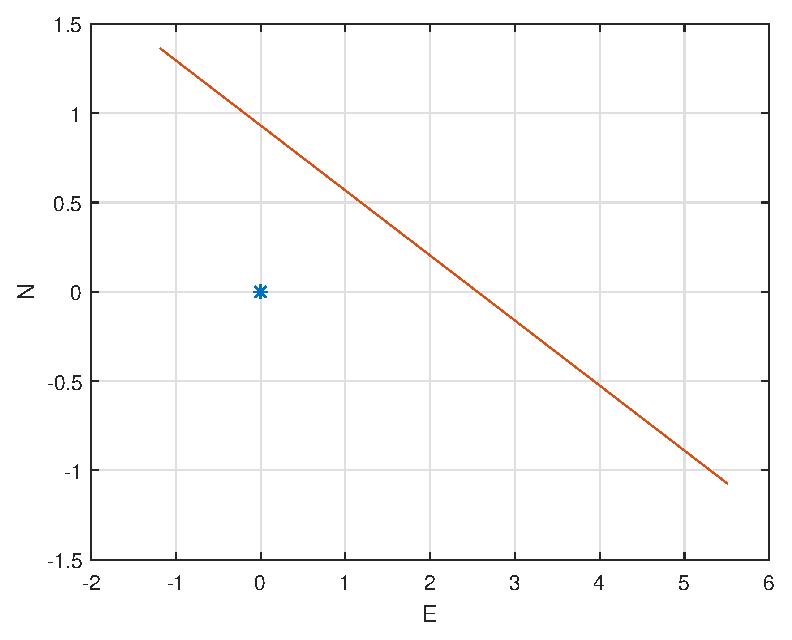
\includegraphics[width=0.8\textwidth, keepaspectratio=true]{../../trials/kinematic_output.eps}}
    \caption{Graph showing the line the camera captures when the plane is positioned in the origin with an altitude of $10m$, and $\phi=-10$, $\theta=-5$ and $\psi=20$. The field of view is $20\degree$.}
\end{figure}